% =====================================================================
%  Detekce malárie --- pracovní šablona miniprojektu (Veletrh vědy, FJFI ČVUT)
%
%   TOHLE JE DRAFT. Popisuje SOUČASNÉ řešení (ResNet50 + k-NN baseline).
%     Prepiste casti oznacene "Pro tym:" podle sveho vlastniho reseni
%     (jiný klasifikátor, jiné příznaky, lepší výsledky\dots).
%
%  Kompilace: pdfLaTeX (Overleaf: Menu -> Compiler -> pdfLaTeX).
% =====================================================================
\documentclass[11pt]{article}

\usepackage[utf8]{inputenc}
\usepackage[T1]{fontenc}
\usepackage[czech]{babel}
\usepackage{lmodern}

\usepackage{amsmath}
\usepackage{booktabs}            % kvalitní vodorovné linky v tabulkách
\usepackage{siunitx}             % zarovnání čísel na desetinnou čárku
\usepackage{graphicx}
\usepackage{xcolor}
\usepackage[margin=2.5cm]{geometry}
\usepackage[colorlinks=true,allcolors=blue]{hyperref}
\usepackage[capitalize,nameinlink]{cleveref}

% čeština pro křížové odkazy z cleveref
\crefname{figure}{obrázek}{obrázky}\Crefname{figure}{Obrázek}{Obrázky}
\crefname{table}{tabulka}{tabulky}\Crefname{table}{Tabulka}{Tabulky}
\crefname{section}{sekce}{sekce}\Crefname{section}{Sekce}{Sekce}
\crefname{equation}{rovnice}{rovnice}\Crefname{equation}{Rovnice}{Rovnice}

% české desetinné čárky v číslech siunitx
\sisetup{output-decimal-marker={,}, detect-weight=true, table-number-alignment=center}

% --- Naměřené hodnoty (k-NN baseline, testovací sada). Tým si je nahradí svými. ---
\newcommand{\Ntotal}{27\,558}
\newcommand{\Ntrain}{19\,289}
\newcommand{\Nval}{4\,135}
\newcommand{\Ntest}{4\,134}
\newcommand{\knnK}{31}
\newcommand{\knnAcc}{0{,}77}        % přesnost při prahu 0,5
\newcommand{\knnSens}{0{,}56}       % senzitivita při prahu 0,5
\newcommand{\knnSpec}{0{,}99}       % specificita při prahu 0,5
\newcommand{\knnFN}{904}            % přehlédnutí nemocní při prahu 0,5
\newcommand{\knnTP}{1163}
\newcommand{\knnSensNF}{0{,}74}     % SOUTĚŽNÍ metrika: senzitivita @ spec >= 95 %
\newcommand{\knnAUC}{0{,}93}

\title{\textbf{Detekce parazita malárie v~krevním nátěru pomocí\\
přenosového učení a~metody $k$ nejbližších sousedů}\\[4pt]
\large\textnormal{Pracovní šablona miniprojektu --- upravte podle vlastního řešení}}

% Pro tým: doplňte svá jména a název týmu.
\author{Jméno Příjmení \and Jméno Příjmení\\[2pt]
\small Tým \uv{\dots} \,$\cdot$\, Veletrh vědy \,$\cdot$\, Katedra matematiky FJFI ČVUT}
\date{\today}

\begin{document}
\maketitle

\begin{abstract}
\noindent
Malárie každoročně způsobí zhruba 600\,000 úmrtí, převážně tam, kde chybí vyškolení
patologové schopní rozpoznat parazita pod mikroskopem. Zkoumáme, zda lze tuto úlohu
automatizovat: na veřejném datasetu \Ntotal{} mikroskopických snímků jednotlivých
červených krvinek (Národní institut zdraví, NIH) rozlišujeme buňky zdravé od napadených
parazitem \emph{Plasmodium}. Naše současné řešení nejprve použije zmrazenou konvoluční
neuronovou síť ResNet50 jako extraktor příznaků a~na získaných vektorech klasifikuje
buňky jednoduchou metodou $k$ nejbližších sousedů ($k$-NN). Tento baseline dosahuje na
testovací sadě plochy pod ROC křivkou \knnAUC{}. Současně ukazujeme, proč v~medicíně
nestačí samotná přesnost: při výchozím prahu má model přesnost \knnAcc{}, ale senzitivitu
jen \knnSens{} --- přehlédne tedy bezmála polovinu nemocných. Tato šablona slouží jako
výchozí bod; svůj vlastní, lepší klasifikátor do ní doplníte na vyznačených místech.
\end{abstract}

% =====================================================================
\section{Úvod a~vymezení problému}
\label{sec:uvod}

Malárie zůstává jednou z~nejsmrtelnějších infekčních nemocí: podle Světové zdravotnické
organizace (World Health Organization, WHO) na ni v~roce 2022 zemřelo přibližně 600\,000
lidí~\cite{who2023}. Spolehlivá diagnóza se přitom stále opírá o~tzv. \emph{tlustou kapku}
a~\emph{tenký nátěr} krve, kde laborant pod mikroskopem hledá v~červených krvinkách
parazita \emph{Plasmodium}. Tento postup je pomalý, vyžaduje zkušeného odborníka a~právě
v~oblastech s~nejvyšším výskytem malárie takových odborníků zoufale chybí. Vzniká tak
otázka, kterou řešíme: \emph{lze rozhodnutí \uv{je tahle buňka napadená?} spolehlivě svěřit
algoritmu?}

Klíčovou překážkou pro klasické strojové učení je, že natrénovat rozpoznávač obrazu od
nuly vyžaduje miliony označených snímků a~značný výpočetní výkon. Obojí obcházíme pomocí
\emph{přenosového učení} (transfer learning): převezmeme síť předtrénovanou na milionech
běžných fotografií, využijeme její schopnost \uv{vidět} tvary a~textury, a~doučíme jen malou
rozhodovací část. Konkrétně v~tomto draftu kombinujeme zmrazený extraktor příznaků ResNet50
s~klasifikátorem $k$ nejbližších sousedů a~na datasetu NIH dosahujeme plochy pod ROC křivkou
\knnAUC{}; zároveň zdůrazňujeme, že kvalitu medicínského klasifikátoru je nutné posuzovat
podle senzitivity a~specificity, nikoli podle pouhé přesnosti.

Tento dokument je \textbf{pracovní šablona}. Popisuje výchozí řešení a~jeho vyhodnocení tak,
abyste z~něj mohli vyjít a~nahradit jej vlastním, vylepšeným postupem. Místa, kde to máte
udělat, jsou označena poznámkou \uv{Pro tým}.

\medskip\noindent\textit{Pro tým: do tohoto úvodu doplňte jednou větou, čím se vaše řešení
liší od baseline a~jakého hlavního výsledku dosahuje.}

% =====================================================================
\section{Data}
\label{sec:data}

Pracujeme s~veřejným datasetem \emph{Malaria Cell Images} amerického Národního institutu
zdraví~\cite{rajaraman2018}. Obsahuje \Ntotal{} barevných snímků jednotlivých, již
vysegmentovaných červených krvinek a~je dokonale \emph{vyvážený} --- právě polovina buněk
je napadená parazitem a~polovina zdravá (13\,779 a~13\,779). Vyváženost je důležitá pro
interpretaci výsledků: znamená, že náhodné hádání dává přesnost 50~\%, takže každé zlepšení
nad tuto hranici pochází ze skutečně naučeného rozdílu.

Aby výsledky poctivě měřily zobecnění na nové buňky, rozdělili jsme data na tři části
\emph{stratifikovaně} (se zachováním poměru tříd) a~s~pevným náhodným zrnem: trénovací
sadu (\Ntrain{} buněk), ověřovací sadu (\Nval{} buněk) pro ladění a~výběr modelu, a~skrytou
testovací sadu (\Ntest{} buněk), kterou používáme výhradně pro závěrečné vyhodnocení.
Oddělená testovací sada je zásadní: bez ní bychom snadno vyladili model na konkrétní data
a~přecenili jeho skutečnou kvalitu.

% =====================================================================
\section{Metoda}
\label{sec:metoda}

\subsection{Extrakce příznaků zmrazeným ResNet50}
\label{sec:priznaky}

Protože nemáme dost dat ani času na trénink konvoluční neuronové sítě (convolutional neural
network, CNN) od nuly, použijeme jako \emph{extraktor příznaků} síť ResNet50~\cite{he2016}
předtrénovanou na datasetu ImageNet. Každý snímek buňky nejprve standardně předzpracujeme
(změna velikosti na 224$\times$224 obrazových bodů a~normalizace barev podle ImageNetu)
a~poté jím proženeme sítí, ze které jsme odebrali poslední klasifikační vrstvu. Výstupem je
pro každou buňku vektor \textbf{2048 čísel} --- tzv. \emph{příznaky}, které shrnují, co se
na snímku nachází (tvary, textury, skvrny). Síť přitom necháváme \emph{zmrazenou}: její váhy
se neučí, jen překládá obrázek na čísla. Tím se celá úloha redukuje na klasifikaci vektorů,
kterou zvládne i~slabý počítač během několika sekund.

\subsection{Klasifikace metodou $k$ nejbližších sousedů}
\label{sec:knn}

Jako výchozí klasifikátor jsme zvolili záměrně co nejjednodušší model, abychom získali
poctivou \emph{laťku} (baseline) ke srovnání: metodu $k$ nejbližších sousedů ($k$-nearest
neighbors, $k$-NN)~\cite{cover1967}. Ta se vlastně vůbec netrénuje --- pouze si zapamatuje
trénovací příznaky. Novou buňku zařadí tak, že mezi zapamatovanými najde $k$ nejbližších
(nejpodobnějších v~prostoru příznaků) a~nechá je hlasovat, přičemž bližší sousedé mají větší
váhu; podíl hlasů pro třídu \uv{napadená} bereme jako odhad pravděpodobnosti. Použili jsme
$k=\knnK{}$ sousedů a~před výpočtem vzdáleností příznaky standardizovali (nulový průměr,
jednotkový rozptyl), protože vzdálenosti dávají smysl jen při srovnatelném měřítku jednotlivých
příznaků.

\medskip\noindent\textit{Pro tým: tohle je místo, kde \cref{sec:knn} nahradíte svým řešením
--- například malou trénovanou neuronovou sítí. Popište jeho architekturu a~jak jste ho ladili.}

% =====================================================================
\section{Vyhodnocení}
\label{sec:vyhodnoceni}

\subsection{Proč samotná přesnost nestačí}
\label{sec:metriky}

V~medicíně mají dva druhy chyb zcela odlišnou cenu, a~proto kvalitu klasifikátoru neměříme
pouhou \emph{přesností} (accuracy, podíl správně zařazených buněk). Označme jako pravdivě
pozitivní (true positive, TP) napadené buňky správně označené, falešně negativní (false
negative, FN) napadené buňky chybně prohlášené za zdravé, falešně pozitivní (false positive,
FP) zdravé buňky chybně označené za napadené a~pravdivě negativní (true negative, TN) správně
propuštěné zdravé buňky. Z~nich definujeme dvě klíčové veličiny:
%
\begin{equation}
\mathrm{senzitivita} = \frac{\mathrm{TP}}{\mathrm{TP}+\mathrm{FN}}, \qquad
\mathrm{specificita} = \frac{\mathrm{TN}}{\mathrm{TN}+\mathrm{FP}}\,.
\label{eq:senzspec}
\end{equation}
%
Senzitivita říká, jaký podíl skutečně nemocných model zachytí; nízká senzitivita znamená
přehlížené pacienty, což může stát život. Specificita říká, jaký podíl zdravých model správně
propustí; nízká specificita znamená zbytečné falešné poplachy. Tyto dvě veličiny se navzájem
vyměňují podle zvoleného \emph{prahu}, nad kterým buňku prohlásíme za napadenou; celý
kompromis zachycuje ROC křivka (receiver operating characteristic) a~souhrnně plocha pod
ní (area under the curve, AUC).

Jako hlavní \textbf{soutěžní metriku} jsme zvolili \emph{senzitivitu při specificitě
$\geq 95~\%$} --- tedy kolik nemocných model zachytí, smí-li si dovolit nanejvýš 5~\%
falešných poplachů. Tato metrika přímo kóduje medicínský požadavek \uv{nepřehlédnout nemocného
a~přitom zbytečně nealarmovat} a~odpovídá bodu na ROC křivce při 5~\% falešně pozitivním
poměru.

\subsection{Protokol}
\label{sec:protokol}

Klasifikátor \uv{natrénujeme} (u~$k$-NN pouze zapamatujeme) na trénovací sadě, případnou volbu
prahu provádíme na ověřovací sadě a~všechna níže uvedená čísla měříme na skryté testovací
sadě (\Ntest{} buněk), kterou model při učení nikdy nevidí. Metoda $k$-NN je deterministická,
proto uvádíme výsledky jednoho běhu.

\subsection{Výsledky}
\label{sec:vysledky}

Výsledky baseline shrnuje \cref{tab:vysledky}. Nejnázornější je přitom rozpor mezi přesností
a~senzitivitou: při výchozím prahu $0{,}5$ dosahuje $k$-NN přesnosti \knnAcc{}, ale senzitivity
jen \knnSens{} --- jak ukazuje matice záměn na \cref{fig:confusion}, přehlédne \knnFN{} z~2067
napadených buněk. Vysoká specificita (\knnSpec{}) tu tedy maskuje, že model propustí téměř
polovinu nemocných; samotná přesnost by nás obelhala. Teprve pohled na celou ROC křivku
(\cref{fig:roc}) ukazuje skutečný potenciál modelu: plocha pod ní je \knnAUC{}, a~posuneme-li
práh tak, abychom připustili 5~\% falešných poplachů (specificita 95~\%), vzroste senzitivita
na \knnSensNF{}. To je naše soutěžní skóre, které se budete snažit překonat.

% --- Tabulka výsledků --------------------------------------------------
\begin{table}[t]
\centering
\caption{Výsledky na skryté testovací sadě (\Ntest{} buněk). Přesnost, senzitivita
a~specificita jsou uvedeny při výchozím prahu $0{,}5$; soutěžní metrika je senzitivita
při specificitě~$\geq 95~\%$. Hodnoty jsou z~jednoho deterministického běhu.}
\label{tab:vysledky}
\begin{tabular}{l S[table-format=1.2] S[table-format=1.2] S[table-format=1.2] S[table-format=1.2] S[table-format=1.2]}
\toprule
Metoda & {Přesnost} & {Senzitivita} & {Specificita} & {Senz.\,@\,spec.\,95\,\%} & {AUC} \\
\midrule
ResNet50 + $k$-NN (baseline) & 0.77 & 0.56 & 0.99 & 0.74 & 0.93 \\
Vaše řešení                  & {--} & {--} & {--} & {--} & {--} \\
\bottomrule
\end{tabular}
\end{table}

% --- Obrázky -----------------------------------------------------------
\begin{figure}[t]
\centering
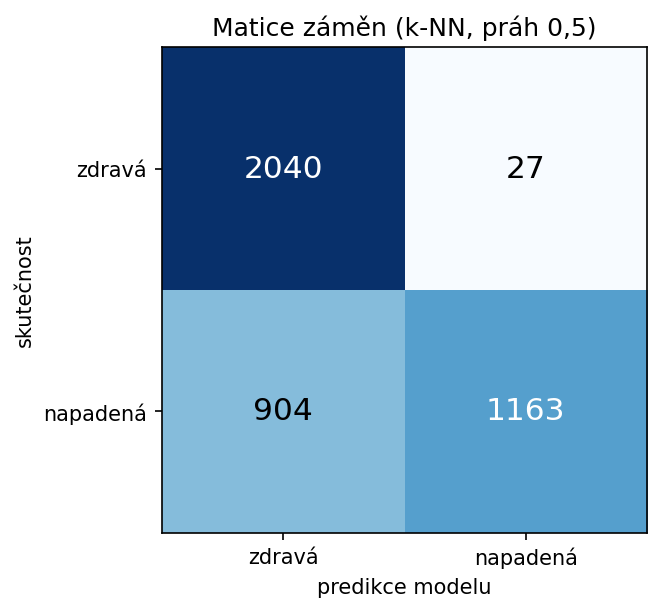
\includegraphics[width=0.55\linewidth]{figs/confusion_baseline.png}
\caption{Matice záměn $k$-NN baseline na testovací sadě při prahu $0{,}5$. Řádky jsou
skutečné třídy, sloupce predikce. Pravý dolní roh (\knnTP{}) jsou správně zachycení nemocní,
levý dolní roh (\knnFN{}) jsou \emph{přehlédnutí} nemocní --- nejdražší typ chyby.}
\label{fig:confusion}
\end{figure}

\begin{figure}[t]
\centering
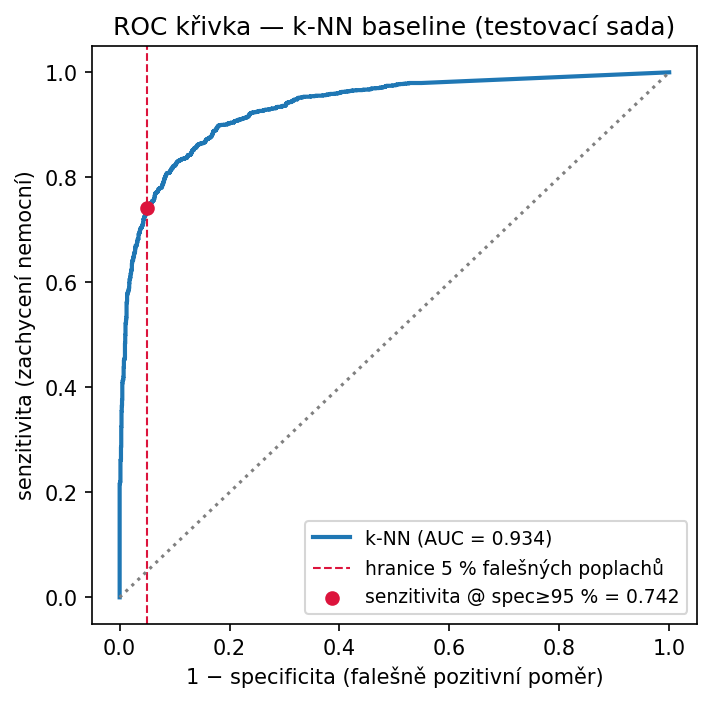
\includegraphics[width=0.6\linewidth]{figs/roc_baseline.png}
\caption{ROC křivka $k$-NN baseline na testovací sadě. Vyznačený bod odpovídá soutěžní
metrice --- nejvyšší senzitivitě dosažitelné při specificitě alespoň 95~\% (tj. nanejvýš
5~\% falešných poplachů).}
\label{fig:roc}
\end{figure}

% =====================================================================
\section{Diskuse}
\label{sec:diskuse}

Slabší výsledek $k$-NN není náhoda, ale důsledek dvou jevů, které stojí za zmínku. Zaprvé,
ve 2048-rozměrném prostoru příznaků přestávají být vzdálenosti spolehlivé --- všechny body se
stávají přibližně stejně vzdálené, takže pojem \uv{nejbližší soused} ztrácí ostrost (tzv.
\emph{prokletí dimenzionality}). Zadruhé, $k$-NN se nic neučí: nedokáže zvážit, které
z~2048 příznaků jsou pro rozlišení parazita důležité, a~bere je všechny stejně. Právě tady
má prostor lépe informovaný model, který se naučí, na čem záleží.

Nezávisle na použitém modelu zůstávají dvě praktická omezení. Skutečné nasazení by se setkalo
s~\emph{doménovým posunem} --- jiný mikroskop, jiné barvení nebo jiná populace pacientů by
mohly přesnost snížit oproti našemu datasetu. A~protože cena přehlédnutého nemocného je vyšší
než cena falešného poplachu, je v~praxi vhodnější model spíše jako nástroj, který lékaře
\emph{upozorní}, než jako konečný rozhodčí.

\medskip\noindent\textit{Pro tým: sem patří rozbor vašich výsledků --- co fungovalo, co ne,
o~kolik jste překonali baseline a~čím to vysvětlujete.}

% =====================================================================
\section{Závěr}
\label{sec:zaver}

Ukázali jsme, že zmrazený ResNet50 jako extraktor příznaků v~kombinaci s~jednoduchým
klasifikátorem $k$ nejbližších sousedů dosahuje na datasetu NIH plochy pod ROC křivkou
\knnAUC{}, a~zdůraznili jsme, proč je v~medicíně nutné hodnotit senzitivitu a~specificitu,
nikoli pouhou přesnost. Tento baseline je výchozím bodem, který má vaše řešení překonat ---
zejména zvýšit senzitivitu při zachování vysoké specificity.

% =====================================================================
\begin{thebibliography}{9}

\bibitem{who2023}
World Health Organization.
\newblock \emph{World Malaria Report 2023}.
\newblock WHO, Ženeva, 2023.

\bibitem{rajaraman2018}
S.~Rajaraman, S.~K. Antani, M.~Poostchi, K.~Silamut, M.~A. Hossain, R.~J. Maude,
S.~Jaeger a~G.~R. Thoma.
\newblock Pre-trained convolutional neural networks as feature extractors toward improved
malaria parasite detection in thin blood smear images.
\newblock \emph{PeerJ}, 6:e4568, 2018.

\bibitem{he2016}
K.~He, X.~Zhang, S.~Ren a~J.~Sun.
\newblock Deep residual learning for image recognition.
\newblock In \emph{IEEE Conference on Computer Vision and Pattern Recognition (CVPR)},
s.~770--778, 2016.

\bibitem{cover1967}
T.~Cover a~P.~Hart.
\newblock Nearest neighbor pattern classification.
\newblock \emph{IEEE Transactions on Information Theory}, 13(1):21--27, 1967.

\end{thebibliography}

\end{document}
